\begin{figure}[!htp]
    \centering
    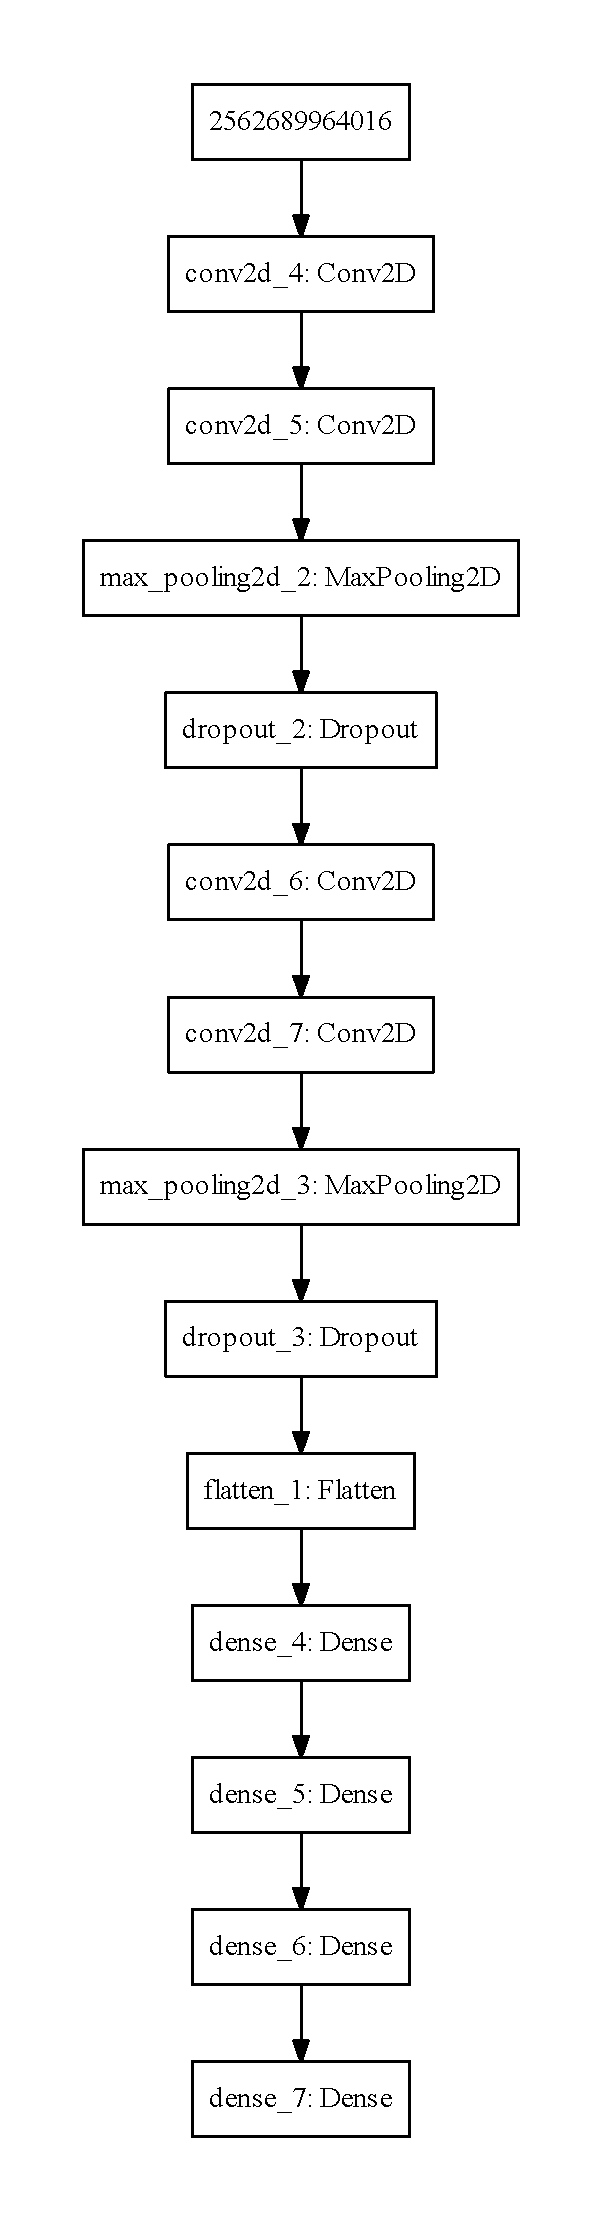
\includegraphics[height=.8\textheight]{Documents/model.pdf}
    \caption{Model Architecture 1}
    \label{fig:model1}
\end{figure}
The model architecture \ref{fig:model1} was implemented using the keras Api in which 2 dimensional 
convolutional layers were added to the sequantial network with intial dimension of image in (224, 224, 3), where width and height of input image is 224 pixels and the rgb channels depth 
are represented by 3. The initial convolutional layers contains 32 input filters with the kernel size of (3, 3) with relu 
activation function. In the network layers followed by first two convolutional layers are polling layer in the 
architecture MaxPooling was used to extract maximum of the input features after applying image filter or kernel 
to the given image of pigmented skin lesions. Furthermore, dropout of 0.4 was used in the network to generialise the 
overall performance of the network and avoid overfitting of data points. 
The next two layers in the networks are also another convolutional layers with 64 image filters and similar relu activation function. Similar fashion as aboved was 
applied to the network with MaxPooling to extract most significant pixels from feature maps followed by the dropout in the network to generialise it.
The features extracted by the convolutional layers are flattened into one dimensional array. The flattened array will be passed to the fully connected layers in the neural network
to process the information. The model contains three dense hidden layers and one output layer in the neural network.
Furthermore, the model architecture was compiled using various hyper-parameters which effects such as learning rate and 
optimiser for the convolutional model which helps in computing the gradient for the loss function to minimise the error in predecting 
category of pigmented skin lesion.

\subsection{Experiments for optimal Model optimiser}
The model architecture at initial stage was compiled using different hyper-parameters
such as optimal optimiser for the neural network and learning rate. These 
hyper-parameters can have impact in finding gradient descent of loss function. Keras libraries 
provides various optimisers such as Adam, SGD and RMSProp Optimiser which 
aims towards reducing the cost function. The model architecture mentioned above was trained for 30 epochs or iteration to 
investigate the optimal optimiser for classification of pigmented skin lesions. The model was trained under learning 
constant rate of 0.001 and loss function of categorical crossentropy because the model has to evaluate the mutiple data classes 
for pigmented skin lesions.
\footnote{\url{https://github.coventry.ac.uk/sareenv/Final-Year-Project/blob/master/Research}}
\pagebreak

\begin{figure}[!htp]
    \centering
    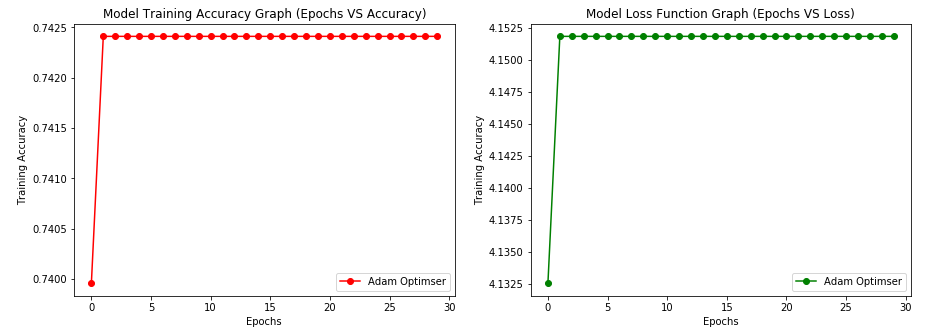
\includegraphics[width=15cm]{Images/Adam Optimiser.png}
    \caption{Model Results obtained with Adam Optimiser}
    \label{fig:adam}
\end{figure}

\paragraph{Adam Optimiser}
The figure \ref{fig:adam} refects the results obtained from training the model using adam optimiser. The figure \ref{fig:adam} shows that model loss function 
is not decreasing and after few epochs there was no improvment in model accuracy which means that adam optimiser is sutaible 
optimiser for model architecture \ref{fig:model1} presented above.

\begin{figure}[!htp]
    \centering
    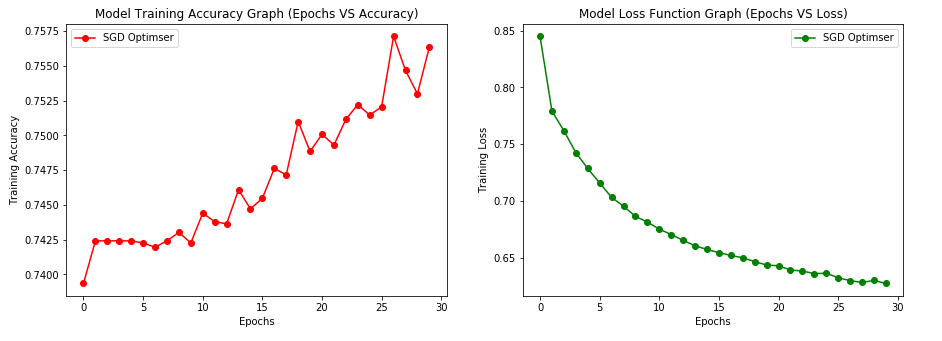
\includegraphics[width=15cm]{Images/SGD.png}
    \caption{Model Results obtained with SGD Optimiser}
    \label{fig:sgd}
\end{figure}

\paragraph{SGD Optimiser}
The figure \ref{fig:sgd} refects the results obtained from training the model using sgd optimiser. The model shows improvment in model 
performance. The training accuracy of model increased over epochs and loss function was decreasing as anticipated as shown in the figure 
\ref{fig:sgd} above.


\begin{figure}[!htp]
    \centering
    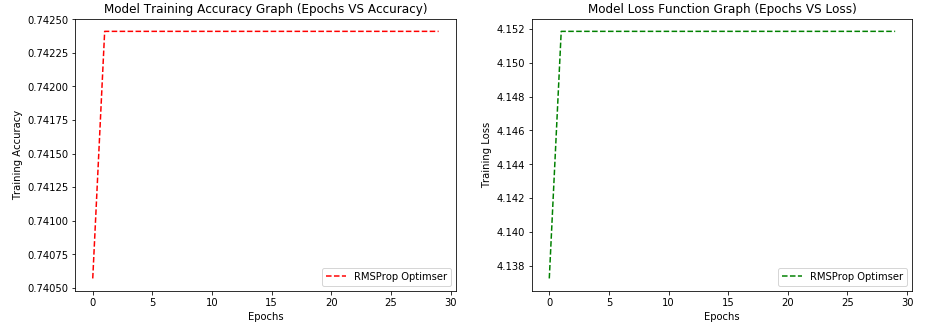
\includegraphics[width=15cm]{Images/rmsprop.png}
    \caption{Model Results obtained with RMSProp Optimiser}
    \label{fig:rms}
\end{figure}

\paragraph{RMSProp Optimiser}
The figure \ref{fig:rms} refects the results obtained from training the model using 'RMSProp' optimiser. The model performance was similar to 
the adam optimiser.Therefore, the SGD optimiser was optimial optimiser for classificaiton model under the constant hyper parameters mentioned above.
the further, experiments performed on convolutional neural network are trained on SGD optimiser.

\footnote{\url{https://github.coventry.ac.uk/sareenv/Final-Year-Project/tree/master/Research}}
